\documentclass[aspectratio=169]{beamer}	  	

\usetheme{Pittsburgh}
\usecolortheme{default}
\usefonttheme[onlymath]{serif}			% para fontes matemáticas
% Enconte mais temas e cores em http://www.hartwork.org/beamer-theme-matrix/ 
% Veja também http://deic.uab.es/~iblanes/beamer_gallery/index.html

% Customizações de Cores: fg significa cor do texto e bg é cor do fundo

\definecolor{cor_titulo_azul}{RGB}{73, 76, 116}
\definecolor{cor_titulo_marrom}{RGB}{155, 138, 107}
\definecolor{cor_block_cinza}{RGB}{200, 200, 200}

\setbeamercolor{normal text}{fg=black}
\setbeamercolor{alerted text}{fg=cor_titulo_azul}
\setbeamercolor{author}{fg=black}
\setbeamercolor{title}{fg=cor_titulo_azul}
\setbeamercolor{institute}{fg=black}
\setbeamercolor{date}{fg=black}
\setbeamercolor{frametitle}{fg=cor_titulo_azul}
\setbeamercolor{framesubtitle}{fg=brown}
%Cor do título
\setbeamercolor{block title}{bg=cor_titulo_marrom, fg=white}
%Cor do texto (bg= fundo; fg=texto)
\setbeamercolor{block body}{bg=cor_block_cinza, fg=black}

% ---
% PACOTES
% ---
\usepackage[alf]{abntex2cite}		% Citações padrão ABNT
\usepackage[brazil]{babel}		% Idioma do documento
\usepackage{color}			% Controle das cores
\usepackage[T1]{fontenc}		% Selecao de codigos de fonte.
\usepackage{graphicx}			% Inclusão de gráficos
\usepackage[utf8]{inputenc}		% Codificacao do documento (conversão automática dos acentos)
\usepackage{txfonts}			% Fontes virtuais
% ---
\usepackage{graphicx}
\usepackage{changepage}
\usepackage{tikz}

\begin{document}

\begin{frame}

\title{\textbf{VISÃO COMPUTACIONAL APLICADA NO
RECONHECIMENTO DE JOGADORES DE FUTEBOL AMERICANO}}

\author[THAYRONE MARQUES SILVA, VINÍCIUS ANDRADE LOPES]
{THAYRONE MARQUES SILVA \and VINÍCIUS ANDRADE LOPES}
 
% \institute{FACULDADES DOCTUM DE IPATINGA
% \par BACHARELADO EM SISTEMAS DE INFORMAÇÃO}
\date{\today
%v-1.9.7
}

\begin{minipage}{1\linewidth}
  \centering
  \begin{tabular}{cc}
    \begin{tabular}{c}
      	\resizebox{.2\linewidth}{!}{
\includegraphics{01-INFO_INICIAIS/doctum-logo-blue.png}}
    \end{tabular}
    &
    \begin{tabular}{c}
      \textbf{FACULDADES DOCTUM DE IPATINGA} \\ \textbf{BACHARELADO EM SISTEMAS DE INFORMAÇÃO}
    \end{tabular}
  \end{tabular}
\end{minipage}

\titlepage

\end{frame}

% \begin{frame}{Sumário}
% \tableofcontents
% \end{frame}

\section{Introdução}

\begin{frame}{Introdução}

\begin{enumerate}
 \item {Visão Computacional;}
 \item {Futebol Americano;}
 \item {Avanço tecnológico.}
\end{enumerate}

\end{frame}

\section{Objetivo Geral}
\begin{frame}
\frametitle{Objetivo Geral}

\begin{block}{}
 Apresentar uma ferramenta que seja capaz de identificar um jogador dentro de campo. Para isso, a identificação será feita através da ferramenta na qual será desenvolvida utilizando visão computacional e a biblioteca de processamento de imagens \textit{OpenCV}.
\end{block}

\end{frame}

\begin{block}{}
\begin{itemize}
\item Classificar as imagens de um jogador de futebol americano e extrair o maior numero de informações.

\item Elaborar um modelo de busca com o conjunto de informações processadas sobre jogadores de futebol americano.

\item Treinar o algoritmo seguindo as configurações do modelo de busca.
   
\item Capturar, através de um dispositivo de entrada de vídeo, as imagens de uma partidade futebol americano.
   
\item Identificar o jogador seguindo o modelo de busca.
   
\item Analisar o percentual de acertos e erros da ferramenta.

\end{itemize}
\end{block}

\section{Justificativa}
\begin{frame}
\frametitle{Justificativa}

\begin{itemize}
\item Crescimento exponencial e utilização em aplicações com soluções específicas.

\item Avanço tecnológico e dispositivos com poder computacional elevado.
   
\item Escalabilidade na utilização da solução para problemas mais complexos.

\item O mercado do futebol americano.

\end{itemize}

\end{frame}

%\section{Organização do Trabalho}
\begin{frame}
\frametitle{Organização do Trabalho}

Este trabalho é composto por cinco capítulos, estruturados da seguinte forma: o \autoref{cap-fundamentos-conceituais} é composto pelos fundamentos conceituais que foram necessários para o entendimento da área de visão computacional. No \autoref{metodologia} foi abordado a metodologia utilizada para a construção deste trabalho.  Subsequente, o \autoref{desenvolvimento} relata todo o desenvolvimento do trabalho, ressaltando todas as etapas de funcionamento, descrição do sistema e requisitos. Por fim, o \autoref{consideracoes_finais} apresenta as considerações finais obtidas com o projeto, seguida das análises dos resultados e possíveis estudos futuros.

\end{frame}

\section{Fundamentos Conceituais}

\subsection{Futebol Americano}
\begin{frame}{Fundamentos Conceituais}{Futebol Americano}
\begin{itemize}
    \item<1> Sua origem foi datada em 1876;
    \item<1> Características;
    \item<1> Recursos para alcançar melhores resultados.
\end{itemize}
\end{frame}

\subsection{Visão Computacional}
\begin{frame}{Fundamentos Conceituais}{Visão Computacional}
\begin{itemize}

\item Se aprimorou a ponto de chegar mais próximo da visão humana e até ser mais eficiente em algumas situações .

\item Abrange todas as técnicas e métodos de processamento de imagem.

\item Foi desenvolvida através da neurofisiologia da visão humana \cite{MARR76}.

\end{itemize}
\end{frame}

\subsection{Reconhecimento facial}
\begin{frame}{Fundamentos Conceituais}{Reconhecimento facial}
\begin{itemize}
    \item<1> Segundo \citeonline{SZELISKI2010}, a área de reconhecimento facial foi a que teve mais sucesso nos dias atuais.
    \item<1> Bibliotecas de reconhecimento.
    \item<1> Reconhecimento de jogadores.
\end{itemize}
\end{frame}

\subsection{Classificação de imagens}
\begin{frame}{Fundamentos Conceituais}{Classificação de imagens}
A classificação de imagem pode ser feita utilizando duas técnicas: supervisionada ou não-supervisionada \cite{LIBERMAN97}.

\begin{enumerate}
    \item<1> \textit{Haar Cascade} - Vetor de características.
    \item<1> \textit{Machine Learning}.
\end{enumerate}
\end{frame}

\subsection{Similaridade}
\begin{frame}{Fundamentos Conceituais}{Similaridade}
\subsubsection{\textit{Similaridade}}

De forma concisa, similaridade consiste em realizar uma buscar dentro de uma imagem específica com o objetivo de reconhecer/encontrar objetos semelhantes a um modelo de busca. Nessas funções de busca por similaridade são utilizados cálculos de vetores de características para realizar as comparações de igualdade \cite{MAIZA2013}.

Os seres humanos possuem uma grande facilidade de reconhecer informações apresentadas de maneira visual, onde consequentemente são capazes, com grande facilidade, de interpretar imagens diversificadas sem grande esforço. Exemplificando esta situação, os seres humanos consegue distinguir de forma fácil a diferença entre um círculo grande e um círculo pequeno, um quadrado grande de um quadrado pequeno, a diferença entre um triângulo e um quadrado de tamanhos idênticos, dentre outros. Conforme \citeonline{SILVA2009} relata em seu artigo, com a tecnologia disponível atualmente para realizar a construção de aplicações capazes de identificar informações dentro de uma imagem ainda é muito ineficiente, quando comparada com a capacidade humana.

Segundo \citeonline{MAIA2013}, algoritmos de similaridade trabalham com métricas que informam o quanto uma imagem é parecida com a outra. Ou seja, pode-se aplicar essas métricas utilizando padrões de buscas a fim de uma análise mais específica. De forma estatística, \citeonline{MAIA2013} completam que possui dois tipos básicos de medidas de similaridade: correlação e coseno. Seguindo o contexto do artigo, a similaridade por correlação entre dois vetores retorna um valor booleano, ou seja, 0 e 1, onde o valor de retorno igual a 1 significa que há uma similaridade forte naquele ponto, ou seja, os valores dos vetores são parecidos e, se o retorno for 0, não existe correlação. No entanto, o autor enfatiza a presença de um retorno igual a -1, no qual a similaridade daquele ponto é inversa ao padrão de busca. Ja a similaridade por coseno é similar a correlação, no qual o retorno também e 0 e 1, porém nesse método é analisado o tamanho do vetor e a formação de um ângulo entre os mesmos. Quanto mais próximo de 1 for o valor, mais similares são os vetores.

\citeonline{MAIZA2013}, \citeonline{MAIA2013} utilizam em seus artigos a função euclidiana para realizar cálculos de distâncias nas estruturas. Essa função utiliza métricas de similaridade para calcular a distância entre dois vetores de características, percorrendo o vetor apenas uma vez. A distância euclidiana entre dois pontos (Xi e Xj) é definida através de uma equação matemática, na qual não faz parte do escopo deste projeto.
\end{frame}

\section{Metodologia}
\begin{frame}
\frametitle{Metodologia}
\label{metodologia}

\end{frame}

\section{Desenvolvimento}
\subsection{Descrição do sistema}
\begin{frame}{Desenvolvimento}{Descrição do sistema}

Através da técnica classificação de imagem, o presente \textit{software} realiza a extração dos padrões de características de uma imagem. Nessa etapa, o sistema passa por um aprendizado de máquina para extrair os padrões de características que são necessária para atender as necessidades do projeto, que é reconhecer um jogador em campo.

\end{frame}

\begin{frame}{Descrição do sistema}
\begin{figure}
    \centering
    \caption{\label{fig_conversao_img}Etapa de extração de características de uma imagem (A) e seu padrão de características (B).}
    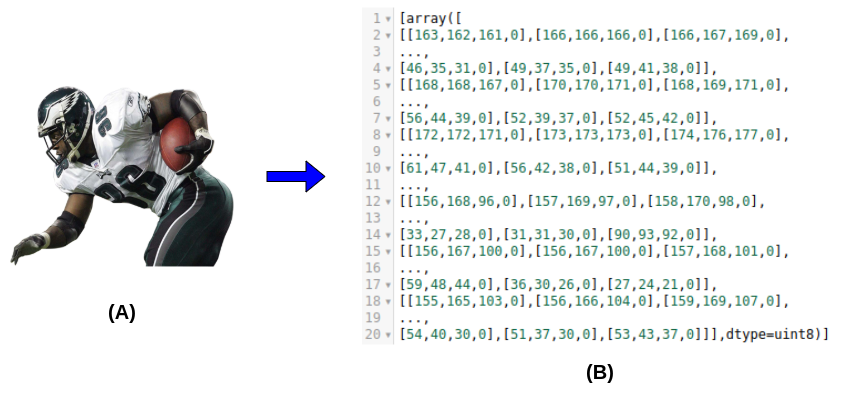
\includegraphics[scale=0.3]{05-SLIDES_DESENVOLVIMENTO/Imagens/conversao-de-imagem.png}
\end{figure}
\end{frame}

\section{Considerações Finais}
\begin{frame}
\frametitle{Considerações Finais}
\label{consideracoes_finais}

\end{frame}


\subsection{Propostas de novos estudos}
\begin{frame}{Considerações Finais}{Propostas de novos estudos}
\begin{itemize}
    \item<1> Processamento dos \textit{frames} do vídeo em um servidor \textit{web}.
    \item<1> Realizar a análise apenas do jogador que esta com a bola em mãos.
\end{itemize}
\end{frame}

\section{Referências}

% --- O comando \allowframebreaks ---
% Se o conteúdo não se encaixa em um quadro, a opção allowframebreaks instrui 
% beamer para quebrá-lo automaticamente entre dois ou mais quadros,
% mantendo o frametitle do primeiro quadro (dado como argumento) e acrescentando 
% um número romano ou algo parecido na continuação.

\begin{frame}[allowframebreaks]{Referências}
\bibliography{references}
\end{frame}

\end{document}
